\begin{figure*}[t]
  \centering
  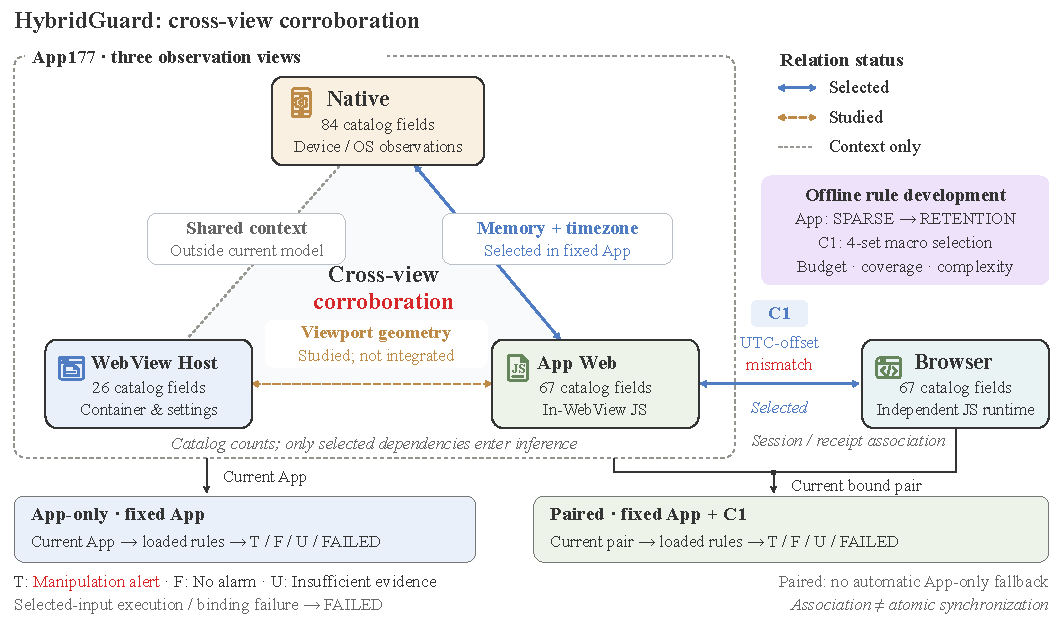
\includegraphics[width=\textwidth]{figures/HybridGuard_overview_triangle.pdf}
  \caption{HybridGuard as a triangle of complementary observation views. Native, WebView Host, and App Web provide device/system, container/settings, and webpage-runtime observations. Solid blue edges denote relations selected in the retained models: Native--App Web memory and timezone relations, and the App Web--independent Browser numeric UTC-offset condition C1. The dashed ochre edge denotes separately studied Host geometry that is not integrated; the arrowless dotted gray edge denotes only shared Native--Host context outside the current App rule pool. Arrowed comparison edges identify the views being compared, not bidirectional rule execution or trusted ground truth. The App detector combines within-view rules with selected cross-view relations. Offline development applies App SPARSE selection and RETENTION, followed by constrained macro-detection selection over four cross-endpoint sets. Separate App-only and paired interfaces load fixed models and read only current inputs. T denotes a manipulation alert, F no alarm, and U insufficient evidence; execution or binding failures in selected inputs take precedence as FAILED. Paired inference has no automatic App-only fallback. Field counts describe catalogs, binding IDs are not detection features, and association does not imply atomic synchronization.}
  \Description{Native, WebView Host, and App Web form a triangle. Selected memory and timezone comparisons use a solid blue edge; separately studied geometry uses a dashed ochre edge. The arrowless dotted gray edge denotes shared context only. The independent Browser is outside the triangle and connected to App Web by C1. Offline development is separate from the two current-input interfaces.}
  \label{fig:hybridguard-overview}
\end{figure*}
